\documentclass[onecolumn]{article}
\usepackage{graphicx}
\usepackage{float}
\restylefloat{figure}
\begin{document}

\title{Curves of infinite length but indistinguishable from a line piece?}

\author{Arjen Markus}

\maketitle

\subsection*{Introduction}
Infinity tends to surprise us. Take fractals or space-filling curves. Or
the theorem by Riemann that the order in which you sum the terms of a
conditionally converging series matters for the outcome.

This short note is also about infinity, but in the form of a simple-looking
geometric riddle. It involves the construction of a curve via an infinite
iterative process whose length can take any value you want but which is not
distinguishable from an ordinary line piece. I am not sure where I go wrong --
if I go wrong, but, well, here it is.

\subsection*{Construction of a curve}
Consider the following curve:
\begin{figure}[H]
\begin{center}
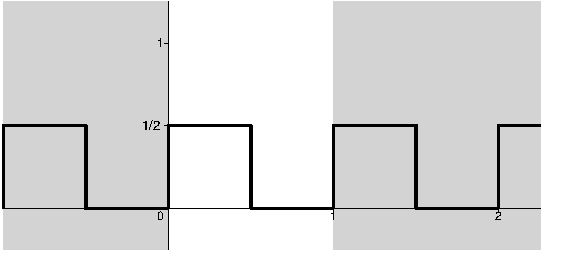
\includegraphics{simple-curve1.pdf}
\label{SimpleCurve1}
\end{center}
\end{figure}

The part we are interested in is the part with \(0 \leq x < 1\) (the area
with the white background in the picture, but excluding the vertical piece at
\(x = 1\)). Its length is 2: the two horizontal pieces are each \(\frac{1}{2}\)
long and the two vertical pieces likewise. Now we can apply a simple linear map
to bring in more "steps": \((x,y) \mapsto (\frac{1}{2}x,\alpha y)\). With
\(\alpha = \frac{1}{2}\) we get the solid line in the figure below and with
\(\alpha = \frac{2}{3}\) we get the dashed curve:
\begin{figure}[H]
\begin{center}
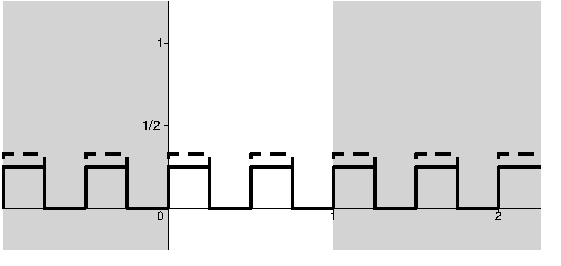
\includegraphics{simple-curve2.pdf}
\label{SimpleCurve1}
\end{center}
\end{figure}

The length of the two curves is: 2 for \(\alpha = \frac{1}{2}\) and
\(2 \frac{1}{3}\) for \(\alpha = \frac{2}{3}\).

We can continue this mapping indefinitely and the result is that the length
stays the same or grows indefinitely:
\begin{table}[H]
\center
\begin{tabular}{ccc}
Step & \(\alpha = \frac{1}{2}\) & \(\alpha = \frac{2}{3}\)                        \\
\hline
\vspace{0.1\baselineskip} \\
1    & \(1 + 4 \cdot \frac{1}{2} \cdot \frac{1}{2} = 2\)     & \(1 + 4 \cdot \frac{1}{2} \cdot \frac{2}{3} = 2 \frac{1}{3}                   \) \\
2    & \(1 + 8 \cdot \frac{1}{2} \cdot \frac{1}{4} = 2\)     & \(1 + 8 \cdot \frac{1}{2} \cdot \bigl( \frac{2}{3} \bigr)^2 = 2 \frac{7}{9}    \) \\
3    & \(1 + 16 \cdot \frac{1}{2} \cdot \frac{1}{8} = 2\)   & \(1 + 16 \cdot \frac{1}{2} \cdot \bigl( \frac{2}{3} \bigr)^3 = 3 \frac{10}{27} \) \\
n    & \(1 + 2^{n-1} \cdot \frac{1}{2} \cdot \bigl( \frac{1}{2} \bigr)^n = 2\) & \(1 + 2^n \cdot \frac{1}{2} \cdot \bigl( \frac{2}{3} \bigr)^n = 1 + \frac{1}{2} \cdot \bigl( \frac{4}{3} \bigr)^n \)  \\
\hline
\end{tabular}
\end{table}

With the iteration number \(n\) going to infinity the length for \(\alpha = \frac{2}{3}\)
goes to infinity too, but for \(\alpha = \frac{1}{2}\) the length remains
constant. With an \(\alpha\) lower than \(\frac{1}{2}\) the length will approach
1. The height of the "steps" is decreasing by a factor \(\alpha\) with
each iteration.

The case of \(\alpha = \frac{1}{2}\) is clearly special, since the length
can be tuned to any value. If we use a different initial height \(h\) for the
steps, we can get any finite length for the case \(\alpha = \frac{1}{2}\) we
want. The length would be: \(1 + 2h\).

\subsection*{The limit curve}
As we continue the mapping, the height becomes less and less (for any factor
\(\alpha\) lower than 1, that is). The end result is a curve that can not be
distinguished from a straight line piece -- but the length is still strictly
larger than the length of that line piece! Note that this is worse than the
construction of a Koch snowflake. That gives a curve of infinite length too, but
at least it does not approach a smooth curve.

The problem quite possibly is that we use the limit process in an inappropriate
way.
\end{document}
